\documentclass{article}

\usepackage{Sweave}
\begin{document}
\Sconcordance{concordance:blix_sweave.tex:blix_sweave.Rnw:%
1 14 1 1 2 1 0 3 1 4 0 1 2 3 1}

\input{blix_Sweave-concordance}

\title{A Minimal Example - blix\_sweave.Rnw}
\author{Yihui Xie}
\maketitle
We examine the relationship between speed and stopping
distance using a linear regression model:
$Y = \beta_0 + \beta_1 x + \epsilon$.


\begin{Schunk}
\begin{Sinput}
> par(mar = c(4, 4, 1, 1), mgp = c(2, 1, 0), cex = 0.8)
> plot(cars, pch = 20, col = 'darkgray')
> fit <- lm(dist ~ speed, data = cars)
> abline(fit, lwd = 2)
\end{Sinput}
\end{Schunk}
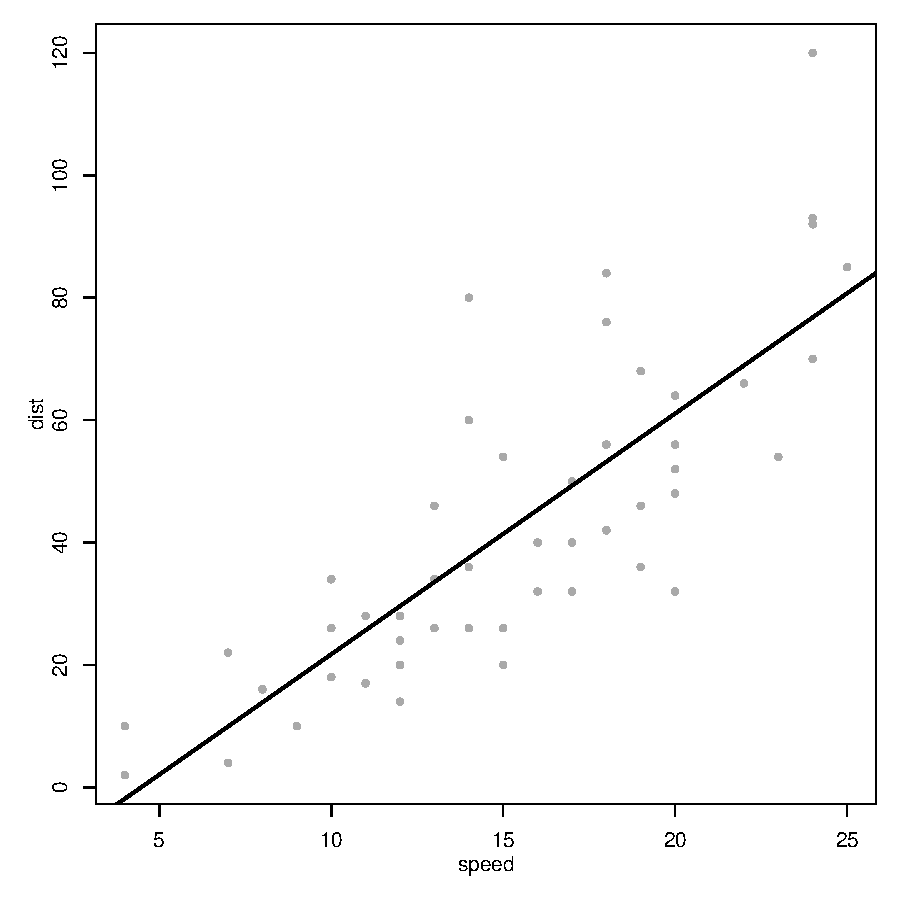
\includegraphics{blix_sweave-model}

The slope of a simple linear regression is
3.93240875912408.
\end{document}
